% interactcadsample.tex
% v1.03 - April 2017

\documentclass[]{interact}

\usepackage{epstopdf}% To incorporate .eps illustrations using PDFLaTeX, etc.
\usepackage{subfigure}% Support for small, `sub' figures and tables
%\usepackage[nolists,tablesfirst]{endfloat}% To `separate' figures and tables from text if required

\usepackage{natbib}% Citation support using natbib.sty
\bibpunct[, ]{(}{)}{;}{a}{}{,}% Citation support using natbib.sty
\renewcommand\bibfont{\fontsize{10}{12}\selectfont}% Bibliography support using natbib.sty

\theoremstyle{plain}% Theorem-like structures provided by amsthm.sty
\newtheorem{theorem}{Theorem}[section]
\newtheorem{lemma}[theorem]{Lemma}
\newtheorem{corollary}[theorem]{Corollary}
\newtheorem{proposition}[theorem]{Proposition}

\theoremstyle{definition}
\newtheorem{definition}[theorem]{Definition}
\newtheorem{example}[theorem]{Example}

\theoremstyle{remark}
\newtheorem{remark}{Remark}
\newtheorem{notation}{Notation}

% see https://stackoverflow.com/a/47122900

% Pandoc citation processing

\usepackage{hyperref}
\usepackage[utf8]{inputenc}
\def\tightlist{}


\begin{document}

\articletype{Preprint}

\title{Continuing COVID-19 Vaccination of Front-Line Workers in BC with
the AstraZeneca Vaccine: Benefits in the Face of Increased Risk for
Prothrombotic Thrombocytopenia}


\author{\name{Amin Adibi$^{a}$}
\affil{$^{a}$Respiratory Evaluation Sciences Program, Faculty of
Pharmaceutical Sciences, University of British Columbia, Vancouver, BC,
Canada}
}

\thanks{CONTACT Amin
Adibi. Email: \href{mailto:amin.adibi@ubc.ca}{\nolinkurl{amin.adibi@ubc.ca}}}

\maketitle

\begin{abstract}
Recently, the National Advisory Committee on Immunization (NACI)
recommended against using the AstraZeneca COVID-19 vaccine pending
further review of the risk for Vaccine-Induced Prothrombotic Immune
Thrombocytopenia (VIPIT). Using straightforward calculations and based
on current evidence, we propose that even if the risk is found to be
causally related to the AstraZeneca vaccine, the benefits of continuing
immunization of essential workers with AstraZeneca by far outweigh the
risk. We consider the case of British Columbia as an example. The
province is expected to received an addtional 246700 doses of
AstraZeneca vaccine through US and COVAX until April 11th, enough to
provide the first dose of vaccine to all unvacinated front-line
workers.We estimate that if British Columbia continues the front-line
worker vaccination program as many as 600 lives could be saved for an
expected mortalilty of only 1 person, even if all essential workers were
under 55 and assuming the highest estimated rate of 1 in 100,000
currently reported for VIPIT.
\end{abstract}

\begin{keywords}
COVID19; astrazeneca; vaccination; essentialworkers; clots;
thrombocytopenia; harm-benefit; BC
\end{keywords}

\hypertarget{background}{%
\section{Background}\label{background}}

Recently, NACI recommended against using AstraZeneca COVID-19 Vaccine
for Canadians under the age of 55, due to concerns about the incidence
of Vaccine-Induced Prothrombotic Immune Thrombocytopenia (VIPIT) based
on European reports \citep{naci_naci_2021}. On Match 18, 2021, the
European Medicines Agency estimated the incidence of VIPIT at
approximately 1 per 1,000,000 people vaccinated with the AstraZeneca
vaccine \citep{ema_covid-19_2021}. A higher estimated rate of 1 per
100,000 by the Paul-Ehrlich Institut in Germany was published on March
19th \citep{pei_covid-19_2021}. It was this higher rate reported by the
Paul-Ehrlich Institut that led NACI to recommend against using this
vaccine in adults under 55 years old \citep{naci_naci_2021}. BC had
initially slated the AstraZeneca vaccine for outbreak control and
front-line workers vaccination program. on March 29th and following
NACI's recommendation, BC paused using the AstraZeneca vaccine for those
under 60 and put the front-line workers vaccination program on hold.

On April 1st, the UK Medicines \& Healthcare Products Regulatory Agency
updated its own previously reported data to report a total of 22
cerebral venous sinus thrombosis (CVST) and 8 other clot-related events
from 18.1 million doses of the AstraZeneca vaccine (total incidence rate
1 in 600,000) \citep{mhra_coronavirus_2021}.

Canadian provinces are expected to receive 1.5 million doses of the
AstraZeneca vaccine from the US and another 316,800 doses from the COVAX
program between now and April 11th
\citep{government_of_canada_vaccines_2021}. British Columbia expects to
receive 246,700 doses from these two AstraZeneca deliveries, enough to
finish providing the first dose to all remaining front-line workers.

The 300,690 doses of Pfizer-BioNTech and 105,900 doses of Moderna
vaccines expected within the same time frame are currently allocated for
the priority groups, indigenous population, and age-based vaccination
campaign currently vaccinating those in their 70s. The AstraZeneca
vaccine was initially slated for essential workers due to its easier
handling and storage requirements. If it is logistically possible to
switch the vaccine allocation for above 55 years old age groups to the
AstraZeneca vaccine and use either Pfizer-BioNTech or Moderna vaccines
for younger front-line workers without delay, that might be the
preferred approach. However, if that is not logistically feasible, one
might ask whether the benefits of deploying the AstraZeneca vaccine for
front-line workers outweigh the rate but serious risk for VIPIT.

Harm-benefit of the administering the AZ doses to younger front-line
workers can be analyzed from either a societal or a personal
perspective. From a societal perspective and assuming a utilitarian
framework, we can estimate compare outcomes such as deaths, life years
lost, or Quality-Adjusted Life Years (QALYs) under different scenarios.
However, a net-beneficial intervention at the societal level does not
necessary translate to a net-benefit at the personal level, as the those
who carry the burden of risk may be different from those who are likely
to benefit from the intervention.

Whether explicitly stated or not, the choice of the outcome is affected
by value judgments as well. Choosing life-years lost as an outcome, for
instance, favours younger people. To make things more complex, roll-out
decisions can get tangled in all sorts of societal issues, including
public trust in not only COVID-19 vaccines but vaccine hesitancy in
general. Ultimately, in dynamic situations like this where the evidence
is uncertain and evolving, vaccine roll-out decision are judgment calls
that need to take a complex network of medical, epidemiological,
ethical, logistics, and societal considerations into account.

Here, we provide a preliminary harm-benefit analysis of immediate
vaccination of all front-line workers with the AstraZeneca COVID-19
vaccine. We based our analysis on mortality alone, and explore the risk
both from a societal and personal perspective, and touch on some
important ethical and practical considerations.

\hypertarget{methods}{%
\section{Methods}\label{methods}}

\hypertarget{covid-19-transmission-model}{%
\subsection{COVID-19 Transmission
Model}\label{covid-19-transmission-model}}

We estimated benefits of the AstraZeneca COVID-19 matrix using a
BC-specific COVID-19 compartmental model by Mulberry and colleagues that
takes into account transmission, age-based contact structure, front-line
worker status, and rising \(R_0\) due to variants of concern
\citep{mulberry_vaccine_2021}. The Mulberry model itself was based on
the transmission model by Bubar et al \citep{bubar_model-informed_2021}.

We ran the model from January 2021 to September 2021, when we expect the
vaccination campaign to conclude.

\hypertarget{results}{%
\section{Results}\label{results}}

\hypertarget{harm-benefit-from-a-societal-perspective}{%
\subsection{Harm-Benefit From A Societal
Perspective}\label{harm-benefit-from-a-societal-perspective}}

Assuming that BC allocates all 246,700 doses to front-line workers, we
can estimate the expected number of deaths due to VIPIT,
\(E(death)_{VIPIT}\), as shown below. To err on the side of caution, we
assume that each dose of the vaccine is independently associated with
the risk for VIPIT and that all recipients are under 55 and as such at
higher risk for VIPIT. We also assume that there is enough uptake that
BC is able to administer all these doses.

\[
E(death)_{VIPIT}  = d \times P(VIPIT|AZ) \times P(death|VIPIT, AZ)
\] where \(d\) is the number of doses administered, \(P(VIPIT|AZ)\) is
the risk of VIPIT after receiving each dose, and \(P(death|VIPIT, AZ)\)
is the case fatality for VIPIT.

To err on the side of caution, we will follow NACI's lead and assume the
highest reported rate of VIPIT, which is 1 in 100,000 recipients, so
\(P(VIPIT|AZ) = \frac{1}{100,000}\). On the other hand, as reported by
NACI, case fatality due to VIPIT is currently estimated at 40\% but is
likely to decrease as there will be more awareness and better early
treatment. Again to err on the side of caution, we'll keep the estimate
at 40\%: \(P(death|VIPIT, AZ)=40\%\)

\[
\begin{aligned}
E(death)_{VIPIT} & = d \times \frac{1}{100,000} \times \frac{40}{100} \\
& = 246,700 \times \frac{4}{1,000,000} \\
& \approx 1  
\end{aligned}
\]

If the second dose of the AstraZeneca vaccine is not associated with
increased and renewed risk for VIPIT, given the current evidence our
best estimate for the number of death associated with AstraZeneca
vaccination campaign for front-line workers would be 1. If, however, we
assume that the second dose will pose an additional risk of VIPIT,
delivering an additional 300,000 doses of the AstraZeneca vaccine will
likely double this estimate, for an expected mortality of 2 persons in
BC.

\begin{figure}

{\centering 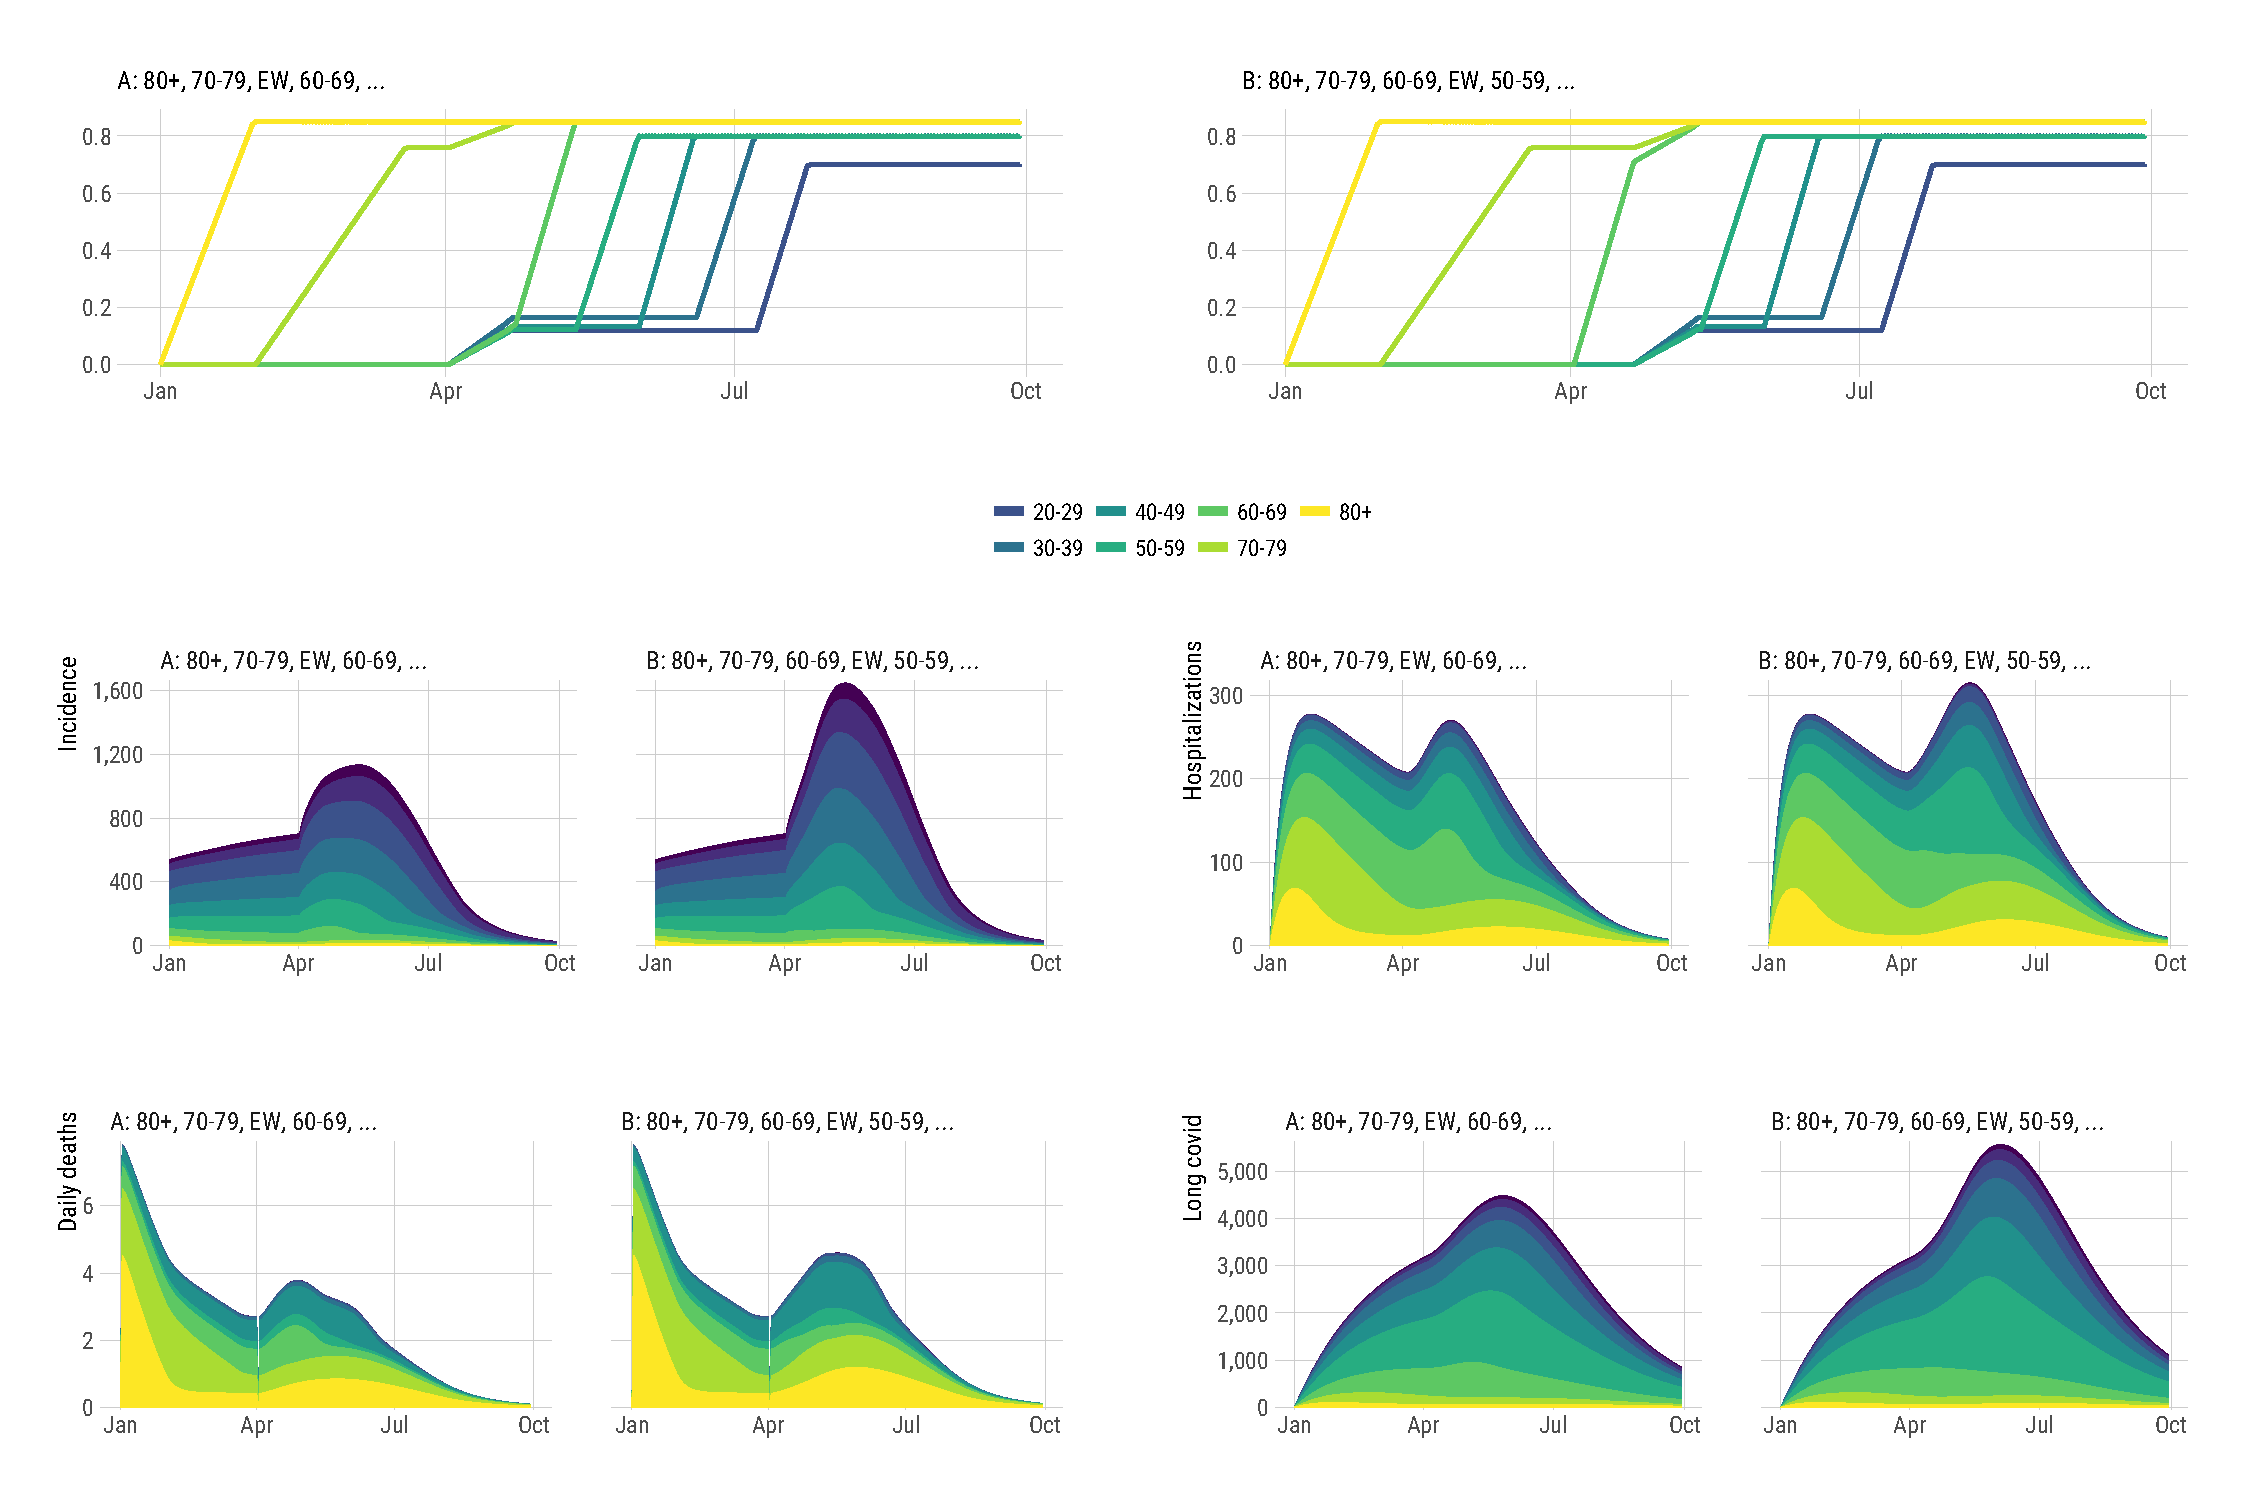
\includegraphics[width=1\linewidth]{./fig-trajectoriesFull} 

}

\caption{your caption}\label{fig:fig1}
\end{figure}

We used a compartmental model of transmission and vaccination of
COVID-19 in BC to estimate benefits of immediately continuing the
front-line workers vaccination program using the AstraZeneca vaccine.

We compared immediately prioritizing essential workers for a vaccine
(Scenario A) and delaying it until after those over 70 are fully
vaccinated (Scenario B).

In our analysis, scenario A led to 39994 fewer cases of COVID-19, 547
fewer hospitalizations, 106 fewer deaths, and 1824 fewer cases of Long
COVID, assuming \(R_0=1.3\) and that vaccine effeteness in preventing
transmission is on average 60\%. Figure 2 shows results for a wider
range of \(R_0\) and efficacy against infection values.

\begin{figure}

{\centering 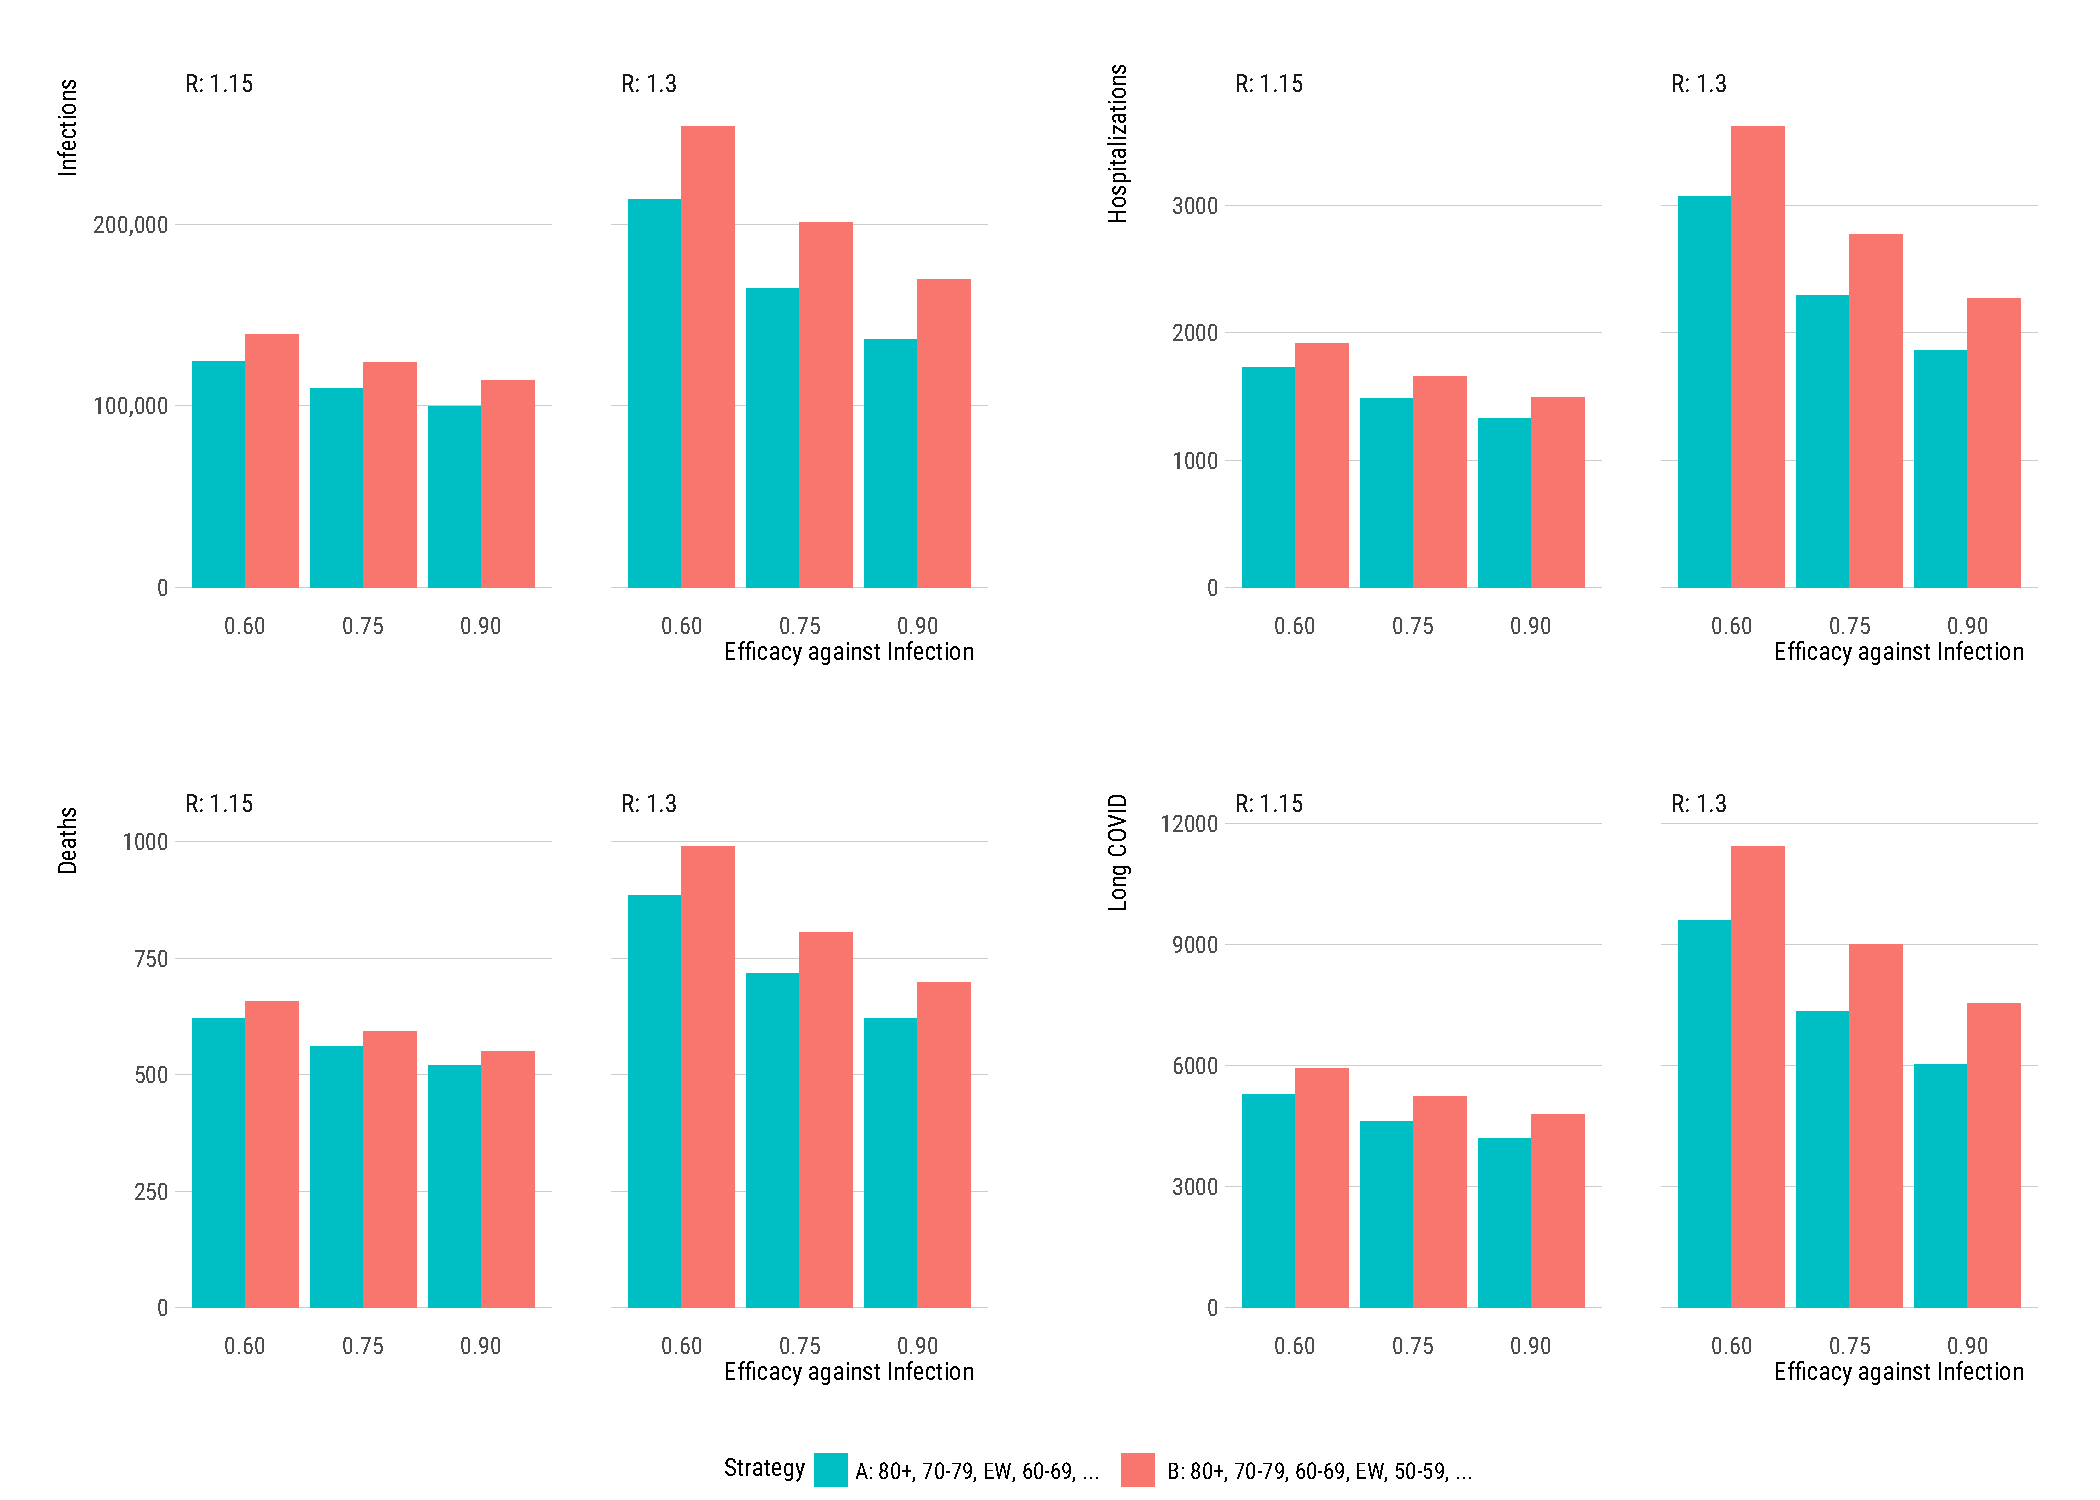
\includegraphics[width=1\linewidth]{./fig-barplots} 

}

\caption{COVID-19 outcomes under different vaccination scenarios}\label{fig:fig2}
\end{figure}

\hypertarget{harm-benefit-from-a-personal-perspective}{%
\subsection{Harm-Benefit From a Personal
Perspective}\label{harm-benefit-from-a-personal-perspective}}

\begin{figure}
\centering
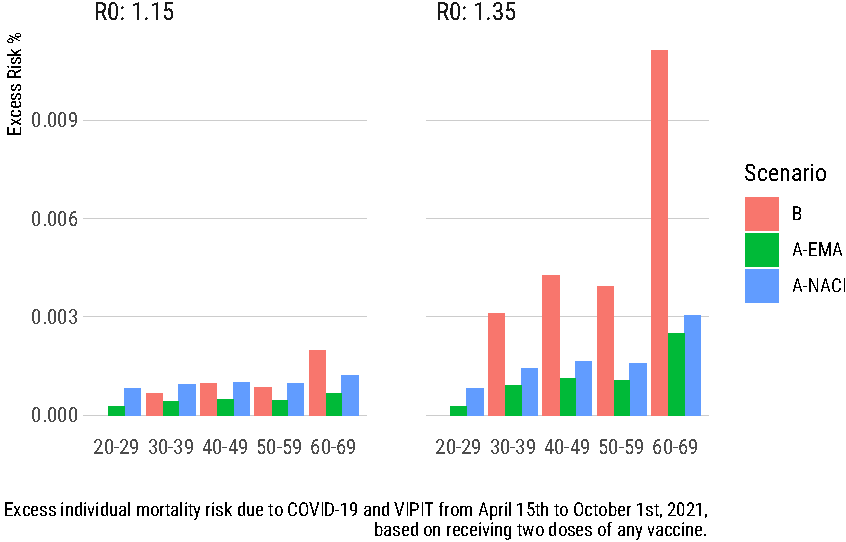
\includegraphics{theCaseforAZ_files/figure-latex/covidvsvipit-1.pdf}
\caption{Mortality risk comparison for different age groups}
\end{figure}

\hypertarget{discussion}{%
\section{Discussion}\label{discussion}}

In its analysis of AstraZeneca vaccine, NACI weighed the risk of adverse
events against the age-stratified risk of mortality due to COVID-19,
pending an overall risk-assessment. However, the benefits of the
AstraZeneca vaccine go beyond preventing COVID-related mortality and
include protection against more common COVID complications in younger
adults including severe disease, hospitalizations, and Long COVID. The
recent sharp decline of COVID-19 cases in the UK suggests that the
AstraZeneca vaccine might also prevent onward transmission of the virus
\citep{our_world_in_data_covid-19_2021}.

The number of confirmed daily COVID-19 cases in the UK has plummeted
from about 60,000 cases a day in early January 2021 when a national
lockdown was imposed and about 3\% of the population had received at
least one vaccine dose, to about 11,000 cases per day on February 22,
2021 when a roadmap to easing lockdowns was announced to about 6000
cases per day on March 8, 2021 when the first phase of easing public
health restrictions was commenced \citep{bbc_lockdown_2021} and has
continuously declined since then to just above 4500 cases as of April 2,
2021 (47\% of the UK population have so far received one dose of a
COVID-19 vaccine). As about half of all vaccine doses administered in
the UK have been AZ vaccines, and based on the estimated AZ vaccine
efficacy of about 76\% against symptomatic COVID-19 and 64\% against any
NAAT-positive COVID-19 infection between 22 and 90 days after first dose
\citep{voysey_single-dose_2021}, and real-world single-dose AZ vaccine
effectiveness of about 60\% against symptomatic COVID-19 and 80\%
against COVID-19 hospitalization
\citep{public_health_england_1public_2021}, it is suggested that the AZ
vaccine is effective in reducing the overall burden of COVID-19.

Potential prevention of onward transmission with the AstraZeneca vaccine
could be especially critical for front-line workers during the current
wave of COVID cases. Of note, two recent studies from Toronto, Ontario
have showed that neighborhoods with the highest proportion of essential
workers had per capita COVID-19 case and death rates that were 2.5-3
folds higher than that of neighborhoods with the lowest share of
essential workers
\citep[\citet{rao_disproportionate_2021}]{chagla_characterizing_2021}.

\hypertarget{doing-vs.-allowing-harm}{%
\subsection{Doing vs.~Allowing Harm}\label{doing-vs.-allowing-harm}}

\hypertarget{communications-and-vaccine-hesitancy}{%
\subsection{Communications and Vaccine
Hesitancy}\label{communications-and-vaccine-hesitancy}}

\hypertarget{limitations}{%
\section{Limitations}\label{limitations}}

We did not consider ethical aspects of vaccine roll-out, and factors
such as uptake and vaccine hesitancy, as they were beyond our expertise.
Our analysis is based on currently available estimated rates of 1 in
million to 1 in 100,000 for VIPIT and might need correction should
higher rates of this complication be reported.

We have not considered potential sex differences in the risk for VIPIT.
Although cases identified to date have been predominantly female, it
remains unclear whether this was due to more females receiving the
AstraZeneca vaccine or due to an intrinsic difference in risk.

\hypertarget{conclusions}{%
\section{Conclusions}\label{conclusions}}

dfsf sdf sf

\bibliographystyle{tfcad}
\bibliography{AZVIPIT.bib}




\end{document}
